\begin{figure}
  \centering
  \definecolor{PipelineColor}{rgb}{1.0,0.901,0.805}
\definecolor{TiledColor}{rgb}{0.7,0.9,1.0}
                           
\tikzstyle{ts-algorithm-base}=[rectangle, 
                             draw=black,
                             rounded corners,
                             text centered,
                             minimum height=1.0cm,
                            ]
\tikzstyle{pipeline}=[ts-algorithm-base,
                                  fill={PipelineColor},
                                  minimum width=6cm]

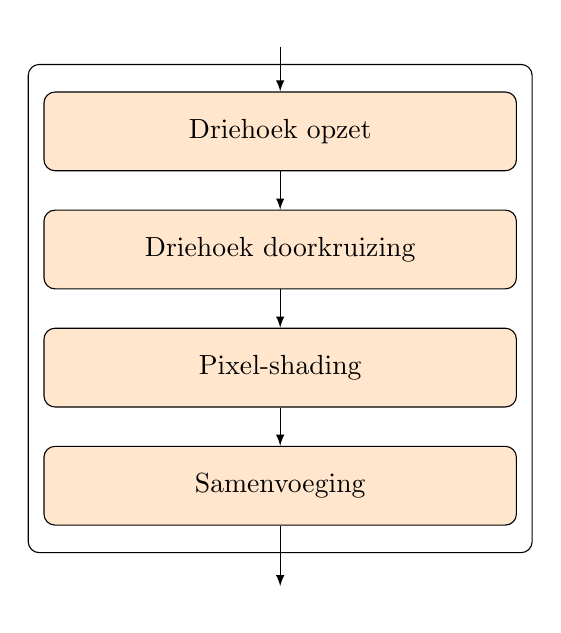
\begin{tikzpicture}
\node at (0cm,    1.2cm) (deferred_step0)     []                  {};
\node at (0cm,   -0.0cm) (deferred_step1)     [pipeline]                  {Driehoek opzet};
\node at (0cm,   -1.5cm) (deferred_step2)     [pipeline]                  {Driehoek doorkruizing};
\node at (0cm,   -3.0cm) (deferred_step3)     [pipeline]                  {Pixel-shading};
\node at (0cm,   -4.5cm) (deferred_step4)     [pipeline]                  {Samenvoeging};
\node at (0cm,   -5.9cm) (deferred_step6)     []                  {};

\node at (0cm, -2.25cm) (l) [rectangle, rounded corners, minimum height=6.2cm, minimum width=6.4cm, draw] {};

\draw[-latex] (deferred_step0) -- (deferred_step1);
\draw[-latex] (deferred_step1) -- (deferred_step2);
\draw[-latex] (deferred_step2) -- (deferred_step3);
\draw[-latex] (deferred_step3) -- (deferred_step4);
\draw[-latex] (deferred_step4) -- (deferred_step6);
\end{tikzpicture}
  \caption{De logische onderverdeling van rasterisatie stap.}
  \label{fig:mgp-rasterisatie}
\end{figure}
